\section{9/12/2019}

\subsection{Recap}

\begin{itemize}
    \item Bounded $\ex \sup_{v \in V} X(v)$ where $X(v)$ concentrates
        and $V$ is finite or could be well approximated by a finite set
        \begin{itemize}
            \item Top eigenvalue of random covariance matrix
            \item VC inequality and symmetrization
        \end{itemize}
    \item Debt: VC-dim of halfspaces is $d+1$ (\cref{eg:half-spaces-vc})
\end{itemize}
Today, we will:
\begin{itemize}
    \item Pay off debt: prove the VC dimension of half spaces is $d+1$
    \item Give a finite-sample analysis of \myref{def:mdf}
    \begin{itemize}
        \item Weaken $\TV$ to $\widetilde{\TV}$
        \item Bound \nameref{prop:mdf-modulus-error-bound} via ``mean crossing lemma''
        \item $\widetilde{\TV}(\tilde{p}, \tilde{p}_n) \to 0$ as $n \to \infty$
    \end{itemize}
\end{itemize}

\subsection{VC dimension of half spaces}

In \myref{eg:half-spaces-vc} we claimed that $vc(\cH) = d+1$ for
the family of half spaces (i.e. linear decision boundaries)
\begin{align}
    \cH = \{ \ind\{\braket{v,x} \geq \tau\} : v \in \RR^d, \tau \in \RR\}
\end{align}
We previously showed it geometrically for the case when $d=2$.
Here, we will generalize this to higher dimensions.

\begin{proposition}[VC dimension of half spaces]\label{prop:vc-dim-half-spaces}
    No $d+2$ set of points in $\RR^d$ can be shattered by any $f \in \cH$.
\end{proposition}

\begin{proof}
    Fix $\{x_i\}_{i=1}^{d+2} \in \RR^d$ distinct.
    We will find two sets $S_+, S_- \subset \{x_1, \ldots, x_{d+2}\}$ such
    that $S_+ \cap S_- = \emptyset$ but $\conv(S_+) \cap \conv(S_-) \neq \emptyset$.
    This is sufficient because every $f = \ind\{\braket{v,x} \geq \tau\} \in \cH$
    can be identified with a half-space (of the points classified $+1$ by $f$)
    \begin{align}
        H = f^{-1}(\{1\}) = \{ x \in \RR^d : \braket{v,x} \geq \tau \}
    \end{align}
    and by convexity of $H$
    \begin{align}
        S_+ \subset H &\implies \conv(S_+) \subset H
    \end{align}
    Hence, if $f$ correctly classifies all of $S_+$ then it must also
    misclassify some $x \in S_+ \cap S_- \subset S_-$.

    Consider the linear system
    \begin{align}
        \sum_{i=1}^{d+2} a_i x_i = 0, \qquad \sum_{i=1}^{d+2} a_i = 0
        \label{eq:9-12-lin-system}
    \end{align}
    or equivalently in matrix form
    \begin{align}
        \underbrace{\begin{bmatrix}
            \vdots & \vdots & \hdots & \vdots \\
            x_1 & x_2 & \hdots & x_{d+2} \\
            \vdots & \vdots & \hdots & \vdots \\
            1 & 1 & \hdots & 1
        \end{bmatrix}}_{(d+1) \times (d+2)} \begin{bmatrix}
            a_1 \\ \vdots \\ a_{d+2}
        \end{bmatrix} = \vec{0}
    \end{align}
    By the rank-nullity theorem, the null-space must have dimension $\geq 1$
    hence there exists at least one solution $\vec{a}$.
    Let
    \begin{align}
        S_+ = \{ i : a_i > 0 \}, \qquad S_- = \{ i : a_i < 0 \}
    \end{align}
    Then by \cref{eq:9-12-lin-system}
    \begin{align}
        \underbrace{\sum_{i \in S_+} \underbrace{\frac{a_i}{A}}_{\in [0,1]} x_i}_{\in \conv(S_+)}
        = \underbrace{\sum_{i \in S_-} \underbrace{\frac{a_i}{A}}_{\in [0,1]} x_i }_{\in \conv(S_-)}
        \qquad \text{where} \quad A = \sum_{i \in S_+} a_i = \sum_{i \in S_-} (-a_i)
    \end{align}
    This gives us a point in $\conv(S_+) \cap \conv(S_-)$.
\end{proof}

\begin{remark}
    The geometric result that ``any set of $d+2$ points in $\RR^d$ can be
    partitioned into two disjoint sets whose convex hulls intersect'' is known
    as \emph{Radon's theorem} on convex sets.
\end{remark}

\subsection{Finite sample analysis of MDF via Generalized KS distance}

Recall \myref{def:mdf} projects $\tilde{p}$ on to $\cG$ under some discrepancy
$D$.  Previously we worked with $D = \TV$, which works fine if $\tilde{p}$ is a
continuous distribution (e.g. $\tilde{p} = \cN(\mu, I)$ in \cref{lem:gauss-tv}).
However, when we only have a finite number of samples we can only form the
empirical distribution
\begin{align}
    \tilde{p}_n
    &= \frac{1}{n} \sum_{i=1}^n \delta_{X_i},
    \qquad X_i \sim \tilde{p}
\end{align}
Here, $\TV$ is inadequate because $\TV(\tilde{p}_n, p) = 1$ almost surely
for any continuous distribution $p$ (this is because $\Pr_{X \sim p}[X = X_i] = 0$)
so it's not clear how to project onto a continuous family such as $\cG_{gauss}$.
Moreover, in many cases $\TV(\tilde{p}_n, \tilde{p}) = 1$ even as $n \to \infty$.

To address this issue, we can consider relaxing $\TV$ to
a weakening $\widetilde{\TV}$ which is more forgiving.
We have two desidirata for $\widetilde{\TV}$:
\begin{enumerate}
    \item The modulus $\fm(\cG, \eps, \widetilde{\TV})$ remains small, so that
        \myref{prop:mdf-modulus-error-bound} still gives a good result
    \item $\widetilde{\TV}(\tilde{p}, \tilde{p}_n) \to 0$ as $n \to \infty$,
        so that $\widetilde{\TV}$ detects convergence of (discrete) empirical
        distributions to a (possibly continuous) population distribution
\end{enumerate}

\begin{remark}
    The two desidirata are competing.
    We want $\widetilde{\TV}$ to be large in
    (1) so that $A = \{ (p,q) \in \cG : \widetilde{\TV}(p,q) \leq \eps \}$ is
    small and hence $\fm = \sup_{(p,q) \in A} L(p, \theta^*(q))$ is small.
    At the same time, in (2) we would like $\widetilde{\TV}$ to be small
    to avoid the failure of $\TV$ in detecting $\tilde{p_n} \to \tilde{p}$
    (e.g. Glivenko-Cantelli ensures that the cumulative distribution functions
    converge uniformly).
\end{remark}

\begin{proposition}\label{prop:mdf-tilde-tv}
    Suppose $\tilde{\TV}$ is a pseudometric such that
    $\widetilde{\TV} \leq \TV$. Let $\hat{\theta}_{\widetilde{\TV}}(p) = \theta^*(q)$ where
    $q \in \argmin_{q \in \cG} \widetilde{\TV}(p, q)$ (the \nameref{def:mdf}
    under $\widetilde{\TV}$). Then
    \begin{align}
        L(p^*, \hat{\theta}_{\widetilde{\TV}}(\tilde{p}_n))
        &\leq \fm(\cG, 2 \eps', \widetilde{\TV})
    \end{align}
    where $\eps' = \eps + \widetilde{\TV}(\tilde{p}, \tilde{p}_n)$
    (and $\widetilde{\TV}(p^*, \tilde{p}) \leq \eps$ as per the conventions
    outlined in \cref{fig:robust-statistics-framework})
\end{proposition}

\begin{proof}
    By \myref{prop:mdf-modulus-error-bound}
    \begin{align}
        L(p^*, \hat{\theta}_{\widetilde{\TV}}(\tilde{p}_n))
        &\leq \fm(\cG, 2 \widetilde{\TV}(p^*, \tilde{p}_n), \widetilde{\TV}, L)
    \end{align}
    Since $\widetilde{\TV}$ is a pseudometric, by the triangle
    inequality
    \begin{align}
        \widetilde{\TV}(p^*, \tilde{p}_n)
        &\leq \underbrace{\widetilde{\TV}(p^*, \tilde{p})}_{\leq \eps} + \widetilde{\TV}(\tilde{p}, \tilde{p}_n)
    \end{align}
\end{proof}

How do we construct $\widetilde{\TV}$?
\begin{definition}[Generalized Kolmogorov-Smirnov distance]\label{def:tilde-tv}
    For a family of functions $\cH = \{ f : \cX \to \RR \}$,
    the \emph{generalized Kolmogorov-Smirnov distance}
    induced by $\cH$ is
    \begin{align}
        \widetilde{\TV}_{\cH}(p, q) &= \sup_{f \in \cH, \tau \in \RR}
        \left\lvert \Pr_p[f(X) \geq \tau] - \Pr_q[f(X) \geq \tau] \right\rvert
    \end{align}
\end{definition}

\begin{remark}
    For $f \in \cH$ and $\tau \in \RR$, if we define the event
    $E_{f,\tau} = \{f(X) \geq \tau\}$ then notice
    \begin{align}
        \widetilde{\TV}_\cH(p,q)
        = \sup_{E_{f,\tau}} \left\lvert
            \Pr_p[E_{f,\tau}] - \Pr_q[E_{f,\tau}]
        \right\rvert
        &\leq \sup_{E~\text{meas}} \left\lvert
            \Pr_p[E] - \Pr_q[E]
        \right\rvert
        = \TV(p,q)
    \end{align}
    So $\widehat{\TV}$ is indeed dominated by $\TV$ as required by
    \cref{prop:mdf-tilde-tv}.
\end{remark}


What $\cH$ should we pick? The answer depends on what we are trying to estimate
(i.e. choice of $L(p, \theta)$). For now, consider mean estimation
(i.e. $L(p,\theta) = \|\theta - \mu(p)\|_2$).
One intuition is that knowledge of the one dimensional
projections ($\ex\braket{v,x}$ for all $v \in \RR^d$) allows us to know
$\ex[X]$, so it's reasonable to consider
\begin{align}
    \cH = \cH_{lin} = \{ x \mapsto \braket{v, x} : v \in \RR^d \}
\end{align}

To bound the modulus, recall that previously if $p, q \in \cG_{\TV}$ are
\nameref{def:resilience}s then \cref{corr:mod-bound-resilient} gave us
\begin{align}
    \TV(p, q) \leq \eps &\implies \|\mu(p) - \mu(q)\|_2 \leq 2 \rho
\end{align}
Similarly, here we will also restrict our distributional assumptions to
be within resilient distributions: $\cG \subset \cG_{\TV}$.

We need to show our two desidirata:
\begin{enumerate}
    \item The modulus is bounded:
    \begin{align}
        p,q \in \cG \subset \cG_{\TV}(\rho, \eps)
        \text{ and } \widetilde{\TV}(p,q) \leq \eps
        \implies \|\mu(p) - \mu(q)\|_2 \leq \sigma = 2 \rho\label{eq:9-12-desidirata-1}
    \end{align}
    \item $\widetilde{\TV}(\tilde{p}, \tilde{p}_n)$ is small, specifically:
    \begin{align}
        \widetilde{\TV}(\tilde{p}, \tilde{p}_n) = O\left(\sqrt{d/n}\right)\label{eq:9-12-desidirata-2}
    \end{align}
\end{enumerate}

\begin{proof}[Proof of \cref{eq:9-12-desidirata-1}]
    Previously we used \nameref{lem:midpoint} to find an $\eps$-deletion
    $r \leq \min\left\{\frac{p}{1 - \eps}, \frac{q}{1 - \eps}\right\}$
    close to both $p$ and $q$ in the sense that
    \begin{align}
            \| \mu(p) - \mu(r) \|_2 \leq \rho
            \text{ and }
            \|\mu(q) - \mu(r) \|_2 \leq \rho
    \end{align}
    After which a triangle inequality completed the proof.

    Unfortunately, we don't know of a way to find a single midpoint distribution
    under $\widetilde{\TV}$.  Instead, we will use the following key property:

    \begin{lemma}[Mean crossing property]\label{lem:mean-crossing-property}
        Suppose $\widetilde{\TV}(p,q) \leq \eps$.
        For any $v \in \RR^d$, there exists $\eps$-deletions $r_p \leq \frac{p}{1 - \eps}$ and $r_q \leq \frac{q}{1 - \eps}$ such that
        \begin{align}
            \ex_{r_q} \braket{v,x} \leq \ex_{r_p} \braket{v,x}
        \end{align}
        In other words, after deleting $\eps$ mass to create $r_q$ and $r_p$, the
        means are shifted such that they cross.
    \end{lemma}

    If we have the $\epsilon$ deletions
    $r_p \leq \frac{p}{1 - \eps}$ and $r_q \leq \frac{q}{1 - \eps}$ from
    \myref{lem:mean-crossing-property}, then
    \begin{align}
        \underbrace{\ex_p \braket{v,x}}_{=\braket{v, \mu_p}}
        &\leq \ex_{r_p}[\braket{v,x}] + \rho &&\text{resilience of $p$} \\
        &\leq \ex_{r_q}[\braket{v,x}] + \rho &&\text{mean crossing} \\
        &\leq \underbrace{\ex_{q}[\braket{v,x}]}_{=\braket{v, \mu_q}} + 2\rho &&\text{resilience of $q$}
    \end{align}
    Hence
    \begin{align}
        \braket{v, \mu_p - \mu_q}
        &\leq 2 \rho
    \end{align}
    for all $\|v\|_2 = 1$. Therefore $\|\mu_p - \mu_q\|_2 \leq 2 \rho$.
\end{proof}

\begin{figure}[H]
    \begin{center}
        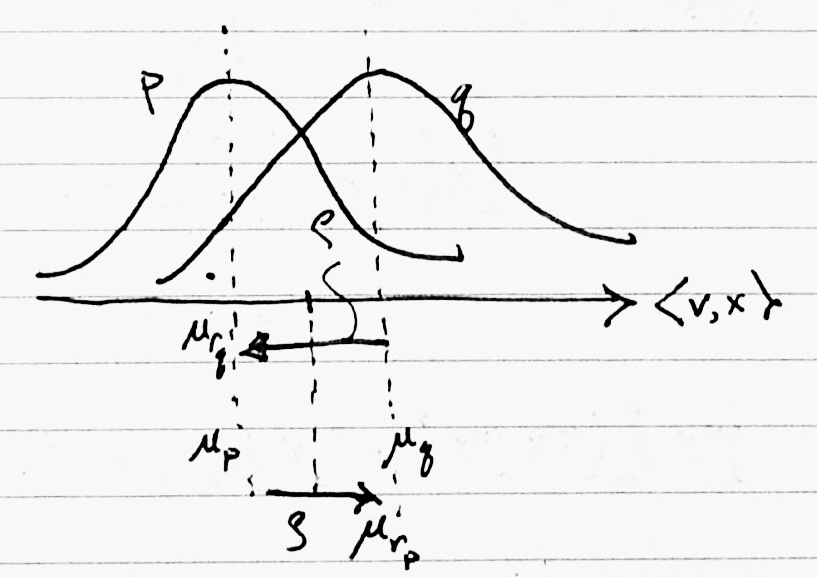
\includegraphics[width=0.4\textwidth]{figures/9-12-1.png}
    \end{center}
    \caption{
        Resilience allows us to perform an $\eps$-deletion to
        move from $\mu_p \to \mu_{r_p}$ and $\mu_q \to \mu_{r_q}$
        and pick up a factor of $+2 \rho$.
        Mean crossing allows us to relate $\mu_{r_p}$ and $\mu_{r_q}$.
    }
    \label{fig:resilience-mean-crossing}
\end{figure}

\begin{proof}[Proof of \nameref{lem:mean-crossing-property}]
    Consider \cref{fig:resilience-mean-crossing}, which visualizes the 1D
    projections of $p$ and $q$ in the $v$ direction.  To make $\braket{v,
    \mu_{r_q}}$ cross over $\braket{v, \mu_{r_p}}$, we would like to shift the
    mean of $q$ to the left and the mean of $p$ to the right as much as
    possible.  Thus, delete $\eps$ mass from the right tail of $q$ (and delete
    the left tail of $p$). Then
    \begin{align}
        \Pr_{r_p}[\braket{v,x} \geq \tau]
        \geq \frac{\Pr_{p}[\braket{v,x} \geq \tau]}{1 - \eps}
        \geq \frac{\Pr_{q}[\braket{v,x} \geq \tau] - \eps}{1 - \eps}
        = \Pr_{r_q}[\braket{v,x} \geq \tau]
    \end{align}
    where the first inequality is because $r_p$ is $p$ with the left
    tail deleted and renormalized by $1-\eps$,
    the second from
    $\Pr_q[\braket{v,x} \geq \tau] - \Pr_p[\braket{v,x} \geq \tau] \leq \widetilde{\TV}(p,q) \leq \eps$,
    and the third from $r_q$ being formed by deleting $\eps$ from the right tail of
    $q$ and renormalizing by $1-\eps$.

    We have shown that the right tail probabilities of $r_p$ are always larger
    than those of $r_q$, i.e. $r_p$ \emph{stochastically dominates} $r_q$.
    As a consequence, $\ex_{r_p}[\braket{v,x}] \geq \ex_{r_q}[\braket{v,x}]$.
\end{proof}

\begin{proof}[Proof of \cref{eq:9-12-desidirata-2}]
    Notice
    \begin{align}
        \widehat{\TV}_{\cH_{\lin}}(p,q)
        &= \sup_{v \in \RR^d, \tau \in \RR} \left\lvert
            \underbrace{\Pr_p[\braket{v,x} \geq \tau] - \Pr_q[\braket{v,x} \geq \tau]}_{\text{max discrepancy on halfspaces}}
        \right\rvert
    \end{align}
    By \nameref{thm:vc-inequality} and \myref{prop:vc-dim-half-spaces}
    \begin{align}
        \widehat{\TV}_{\cH_{\lin}}(\tilde{p}, \tilde{p}_n)
        &\leq O\left(\sqrt{\frac{vc(\text{half spaces})}{n}}\right)
        = O\left(\sqrt{\frac{d + \log \frac{1}{\delta}}{n}}\right)
    \end{align}
    with probability $\geq 1 - \delta$.
\end{proof}

\textbf{Consequences}:
\begin{itemize}
    \item For $(\rho, \eps + O(\sqrt{d/n}))$-resilient distributions, we can estimate mean with error $2 \rho$
    \item For bounded covariance, \cref{corr:mod-cont-cov} gave us
        $\rho(\eps) = O(\sqrt{\eps})$ hence
    \begin{align}
        L(p^*, \tilde{\theta}_{\widetilde{\TV}}(\tilde{p}_n)) 
        \leq O\left(\sqrt{\eps + \sqrt{d/n}}\right)
    \end{align}
    The lower bound $\sqrt{\eps}$ is what we get in the infinite sample $n \to \infty$
    limit, and $\sqrt{d/n}$ when $\eps \to 0$, so we would like $\sqrt{\eps} + \sqrt{d/n}$.
    The slack in the bound comes from $n \gg d / \eps^2$, whereas we would need $n \gg \frac{d}{\eps}$ but this analysis doesnt give it to us.

    \item For sub-Gaussians, $\rho(\eps) = O(\eps \sqrt{\log(1/\eps)})$.
    When $n \gg \frac{d}{\eps^2}$ we get $O(\eps \sqrt{\log (1/\eps)}$.
\end{itemize}
In general, this analysis holds for $n \gg d / \eps^2$: whenever this holds, we can
do as well as if we had infinite data. The analysis is tight in $d$ but loose in $\eps$.

\todo{$\widetilde{\TV}$ similar to Tukey median, may be useful for challenge problem}
